\documentclass[12pt,a4paper]{article}
\usepackage[utf8]{inputenc}
\usepackage{graphicx}
\usepackage{amsmath}
\usepackage{amssymb}
\usepackage{float}
\usepackage{hyperref}
\usepackage{tikz}
\usepackage{pgfplots}
\usepackage{listings}
\usepackage{booktabs}
\usepackage{caption}
\usepackage{subcaption}
\usepackage[margin=1in]{geometry}
\usepackage{xcolor}
\usepackage{algorithm}
\usepackage{algpseudocode}

\pgfplotsset{compat=1.18}

\title{Cache Simulator Implementation and Analysis}
\author{Vijay Balaji $|$ Reeshabh Kotecha}
\date{}

\begin{document}

\maketitle
\begin{abstract}
This report presents the implementation and experimental analysis of a cache simulator. The simulator models an L1 cache with MESI protocol support for a quad-core processor system. Various configurations are tested to analyze cache performance metrics including miss rates, execution cycles, and bus traffic.
\end{abstract}

\tableofcontents
\newpage

\section{Implementation}
% \subsection{System Architecture}
% Add description of the overall system architecture

\subsection{Main Classes and Data Structures}
The cache simulator implementation uses several key data structures and classes to model a multi-core cache system with MESI protocol support:

\begin{lstlisting}[language=C++, caption=Cache State Definitions]
enum class CacheState
{
    INVALID,  // Cache line is invalid or not present
    SHARED,   // Cache line is shared across multiple caches
    MODIFIED, // Cache line has been modified locally
    EXCLUSIVE // Cache line is exclusive to this cache
};

enum class BusState
{
    INVALID,     // Bus is in the process of invalidating
    RWITM,       // Read with Intent to Modify transaction
    RM,          // Read Miss transaction
    TRANSACTION, // Bus is busy with a transaction
    IDLE         // Bus is idle
};
\end{lstlisting}

\begin{lstlisting}[language=C++, caption=Cache Line and Core Structure]
struct CacheLine
{
    int tag;            // Tag bits for address
    CacheState state;   // MESI state of this cache line
    
    CacheLine() : tag(0), state(CacheState::INVALID) {}
};

struct Core
{
    int line;           // Current instruction line
    int core;           // Core ID
    int needsBus;       // Flag indicating need for bus access
    
    // Performance metrics
    int tot_instruc;    // Total instructions executed
    int tot_reads;      // Total read operations
    int tot_writes;     // Total write operations
    int tot_exe_cycles; // Total execution cycles
    int idle_cycles;    // Idle cycles
    int cache_misses;   // Cache miss count
    int cache_evic;     // Cache eviction count
    int writebacks;     // Writeback count
    int bus_invalid;    // Bus invalidation count
    int data_traff;     // Data traffic in bytes
    
    char currentInstruction;  // Current instruction being executed
    int currentAddress;       // Current address being accessed
    
    // Cache structure
    vector<vector<CacheLine>> cache;    // 2D vector representing sets and ways
    vector<vector<int>> cacheLRU;       // LRU tracking for replacement
    vector<pair<char, int>> instructions; // Trace instructions (op, address)
};
\end{lstlisting}

\begin{lstlisting}[language=C++, caption=Bus Class]
class Bus
{
private:
    stack<int> owners;   // Tracks current bus ownership (cores 0-3)
    BusState state;      // Current state of the bus
    int remainingCycles; // Cycles remaining in current transaction
    int source;          // Source of current transaction
    int destination;     // Destination of current transaction
    unsigned int address; // Address for current transaction
    
    int s;               // Number of set index bits
    int E;               // Associativity
    int b;               // Number of block offset bits
    
    int completed[4];    // Completion status for each core
    int cycle;           // Current simulation cycle
    Core cores[4];       // The four processor cores
    
    // Key private methods
    void runCore(int core);              // Process an instruction for a core
    bool isSetFull(int core, unsigned int currentAddress); // Check if a set is full
    CacheState getCacheState(int core, unsigned int currentAddress); // Get cache state
    CacheState getWriteCacheState(int core, unsigned int currentAddress); // Handle write
    CacheState getInvalidCacheState(int core, unsigned int currentAddress); // Find invalid line
    void invalidateAddress(int core, unsigned int currentAddress); // Invalidate caches
    void shareAddress(int core, unsigned int currentAddress); // Share cache lines
    bool containsAddress(int core, int currentAddress); // Check address presence
    void runSnoop(int core); // Run snooping protocol
    void addToCache(int core); // Add data to cache
    void processTransaction(); // Process bus transaction
    bool checkCompletion(); // Check if all cores completed
    bool runCycle(); // Run one simulation cycle
    
public:
    Bus(int s, int E, int b, string appname); // Constructor with cache config and app
    void runApplication(); // Main simulation entry point
};
\end{lstlisting}

\begin{lstlisting}[language=C++, caption=runCycle Method]
bool runCycle()
{
    if (checkCompletion())
        return true;

    processTransaction();
    
    int tempOwner;

    if (owners.empty()) {
        tempOwner = 4;
    } else {
        tempOwner = owners.top();
    }

    if (tempOwner <= 3) {
        runCore(tempOwner);
    }

    for (int i = 0; i < 4; i++)
    {
        if (i != tempOwner)
            runCore(i);
    }

    for (int i = 0; i < 4; i++)
    {
        runSnoop(i);
    }

    return false;
}
\end{lstlisting}

\subsection{Detailed Implementation}
\subsubsection{Other Functions}
% Describe how the cache is structured
\begin{lstlisting}[language=C++, caption=processTransaction Method]
void processTransaction()
{
    remainingCycles--;

    switch (state)
    {
    case BusState::RM:
    case BusState::RWITM:
        state = BusState::TRANSACTION;
        remainingCycles = MEMCYCLES;
        source = 5;
        break;
    case BusState::INVALID:
        state = BusState::IDLE;
        break;
    case BusState::TRANSACTION:
        if (remainingCycles == 0)
        {
            if (destination < 4)
                addToCache(destination);
            if (owners.top() >= 4 && owners.top() <= 7)
                owners.pop();
            state = BusState::IDLE;
        }
        break;
    default:
        break;
    }
}
\end{lstlisting}

\subsubsection{MESI Protocol Implementation}
The cache simulator implements the MESI (Modified, Exclusive, Shared, Invalid) protocol for maintaining cache coherence across the four processor cores. This protocol tracks the state of each cache line and ensures consistency when multiple cores access the same memory locations.

\begin{figure}[H]
    \centering
    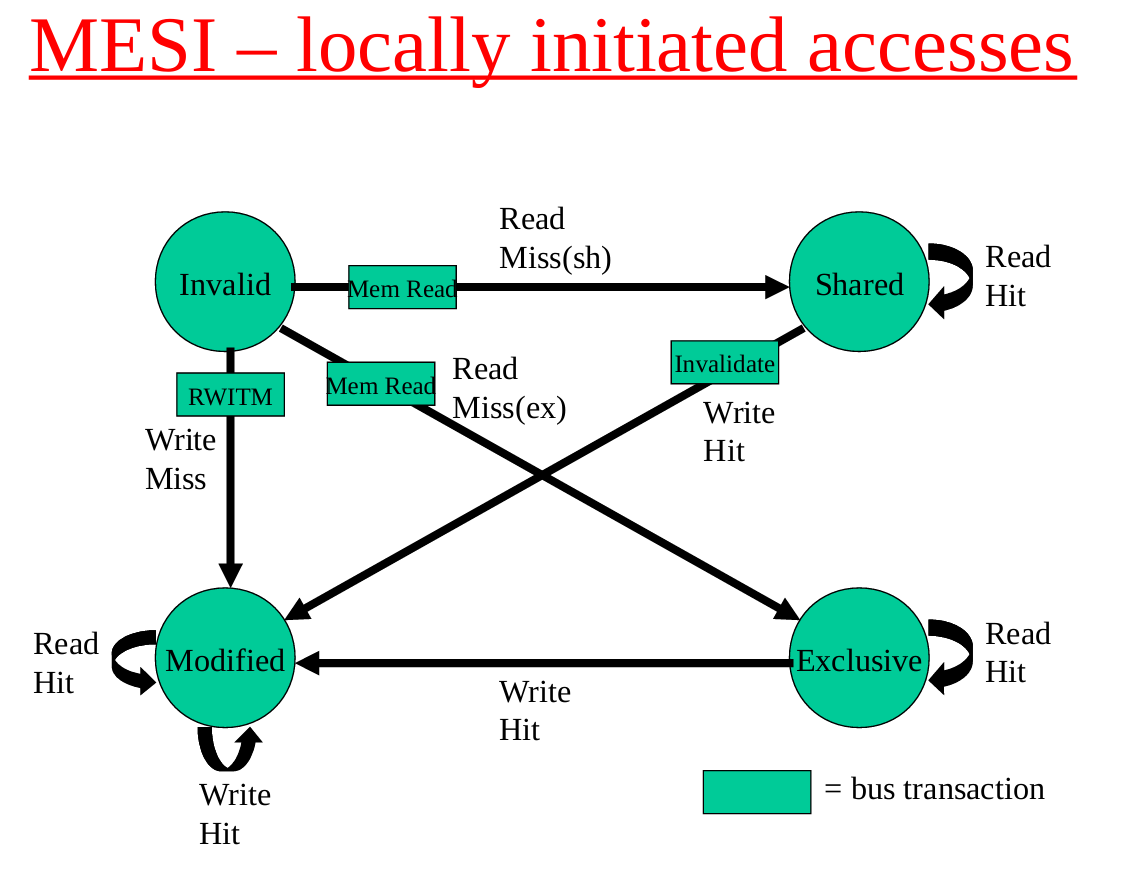
\includegraphics[width=0.9\textwidth]{mesi_local.png}
    \caption{MESI protocol state diagram for locally initiated accesses}
    \label{fig:mesi_local}
\end{figure}

\begin{figure}[H]
    \centering
    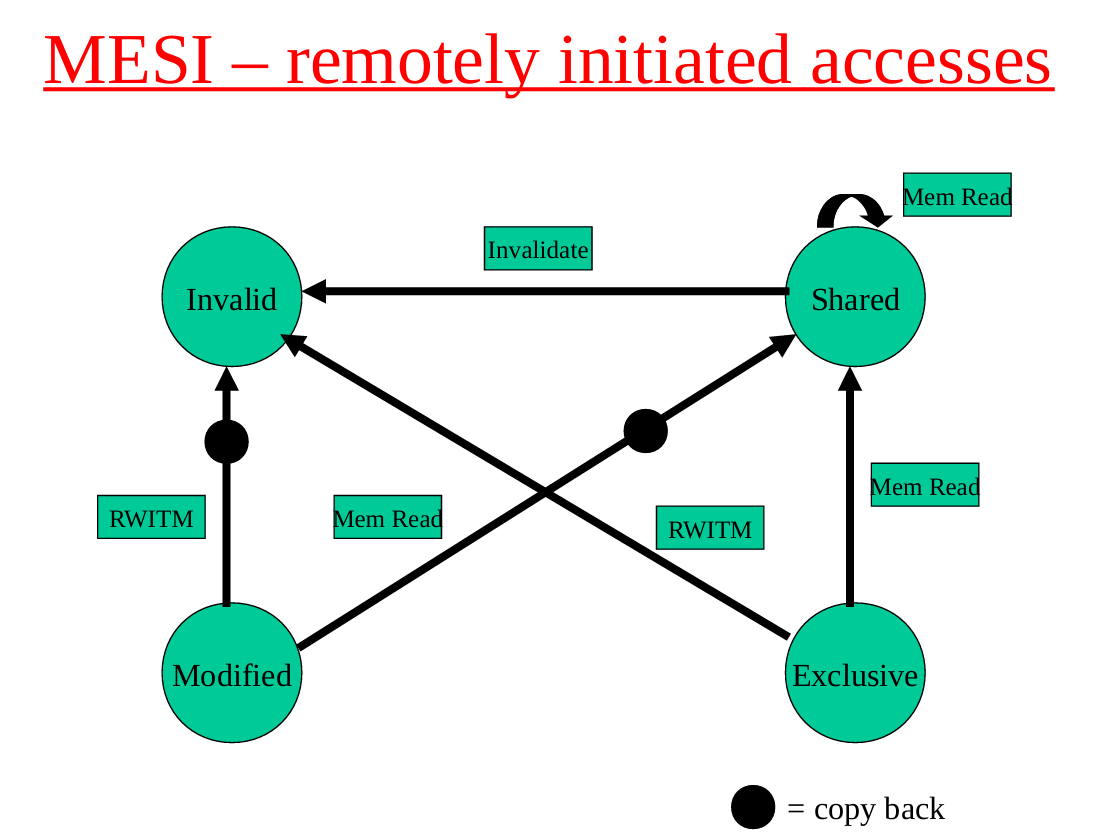
\includegraphics[width=0.9\textwidth]{mesi_remote.png}
    \caption{MESI protocol state diagram for remotely initiated accesses}
    \label{fig:mesi_remote}
\end{figure}

The MESI protocol maintains four possible states for each cache line:
\begin{itemize}
    \item \textbf{Modified (M)}: The cache line is present only in the current cache and has been modified. The data in this cache is newer than in main memory.
    \item \textbf{Exclusive (E)}: The cache line is present only in the current cache but is unmodified. This state transitions to Modified on a write hit without requiring bus transactions.
    \item \textbf{Shared (S)}: The cache line may be stored in other caches and is unmodified. Multiple cores can have the same cache line in Shared state.
    \item \textbf{Invalid (I)}: The cache line is invalid or not present.
\end{itemize}

As shown in the state diagrams, the protocol handles both locally initiated accesses (from the processor) and remotely initiated accesses (from other processors via the bus). Bus transactions like Memory Read, Read With Intent To Modify (RWITM), and Invalidate are used to maintain coherence across all caches.



\subsubsection{Replacement Policy}
% Describe the replacement policy

We have used the LRU Replacement Policy \\
\begin{lstlisting}[language=C++, caption=LRU Replacement Policy]
    CacheState getInvalidCacheState(int core, unsigned int currentAddress)
    {
        unsigned int setIndex = (currentAddress >> b) & ((1 << s) - 1);
        unsigned int tag = currentAddress >> (s + b);

        for (int i = 0; i < E; ++i)
        {
            if (cores[core].cache[setIndex][i].state == CacheState::INVALID)
            {
                cores[core].cache[setIndex][i].tag = tag;
                return CacheState::INVALID;
            }
        }

        cores[core].cache_evic += 1;

        int min = 0;

        for (int i = 0; i < E; i++)
        {
            if (cores[core].cacheLRU[setIndex][i] < cores[core].cacheLRU[setIndex][min])
                min = i;
        }

        cores[core].cache[setIndex][min].tag = tag;

        if (cores[core].cache[setIndex][min].state == CacheState::EXCLUSIVE ||
            cores[core].cache[setIndex][min].state == CacheState::SHARED)
        {
            cores[core].cache[setIndex][min].state = CacheState::INVALID;
            return CacheState::INVALID;
        }
        else if (cores[core].cache[setIndex][min].state == CacheState::MODIFIED)
        {
            cores[core].cache[setIndex][min].state = CacheState::INVALID;
            return CacheState::MODIFIED;
        }
    }
\end{lstlisting}


\section{Experimental Analysis}
\subsection{Experimental Setup}
The cache simulator was tested with various configurations across multiple applications. Each core has its own L1 cache, and they communicate via a shared bus with the MESI protocol to maintain coherence.

\subsection{Parameters}
\begin{table}[H]
\centering
\begin{tabular}{|l|c|}
\hline
\textbf{Parameter} & \textbf{Value} \\
\hline
Set Index Bits & 5 \\
Associativity & 2 \\
Block Bits & 5 \\
Block Size (Bytes) & 32 \\
Number of Sets & 32 \\
Cache Size (KB per core) & 2 \\
Protocol & MESI \\
Write Policy & Write-back, Write-allocate \\
Replacement Policy & LRU \\
\hline
\end{tabular}
\caption{Cache configuration parameters}
\label{tab:parameters}
\end{table}

\subsection{Performance Metrics}
\subsubsection{Cache Miss Rates}

\begin{figure}[H]
\centering
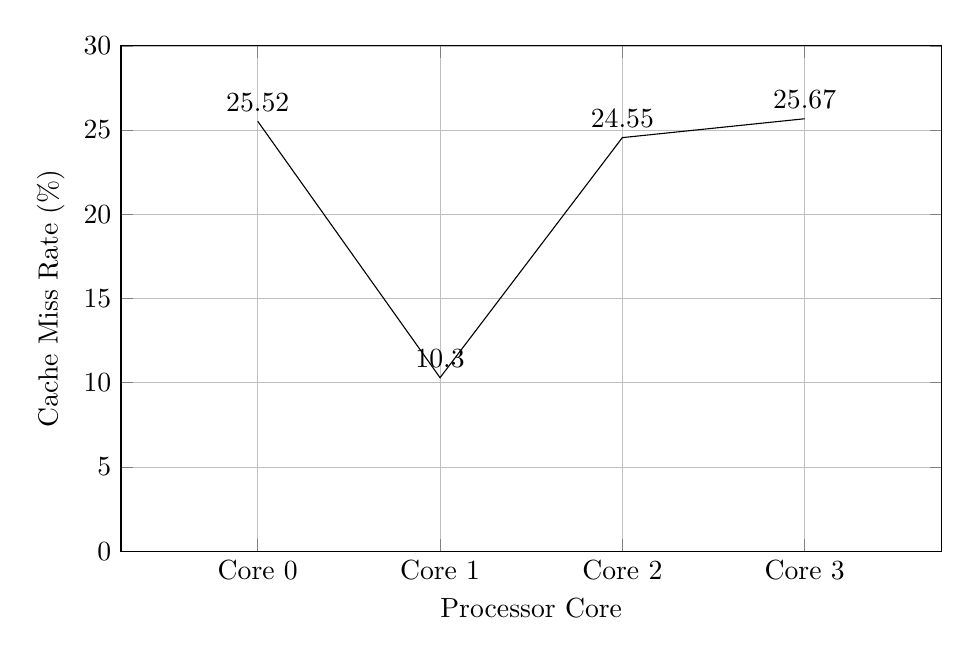
\begin{tikzpicture}
\begin{axis}[
    width=12cm,
    height=8cm,
    ylabel={Cache Miss Rate (\%)},
    xlabel={Processor Core},
    symbolic x coords={Core 0, Core 1, Core 2, Core 3},
    xtick=data,
    ymin=0,
    ymax=30,
    nodes near coords,
    bar width=1cm,
    enlarge x limits=0.25,
    legend pos=north west,
    grid=both,
    grid style={line width=.1pt, draw=gray!10},
    major grid style={line width=.2pt,draw=gray!50},
]
% Replace these values with your actual results
\addplot[] coordinates {
    (Core 0, 25.52)
    (Core 1, 10.30)
    (Core 2, 24.55)
    (Core 3, 25.67)
};
\end{axis}
\end{tikzpicture}
\caption{Cache miss rates across different cores}
\label{fig:miss_rates}
\end{figure}

\subsubsection{Execution Cycles}

\begin{figure}[H]
\centering
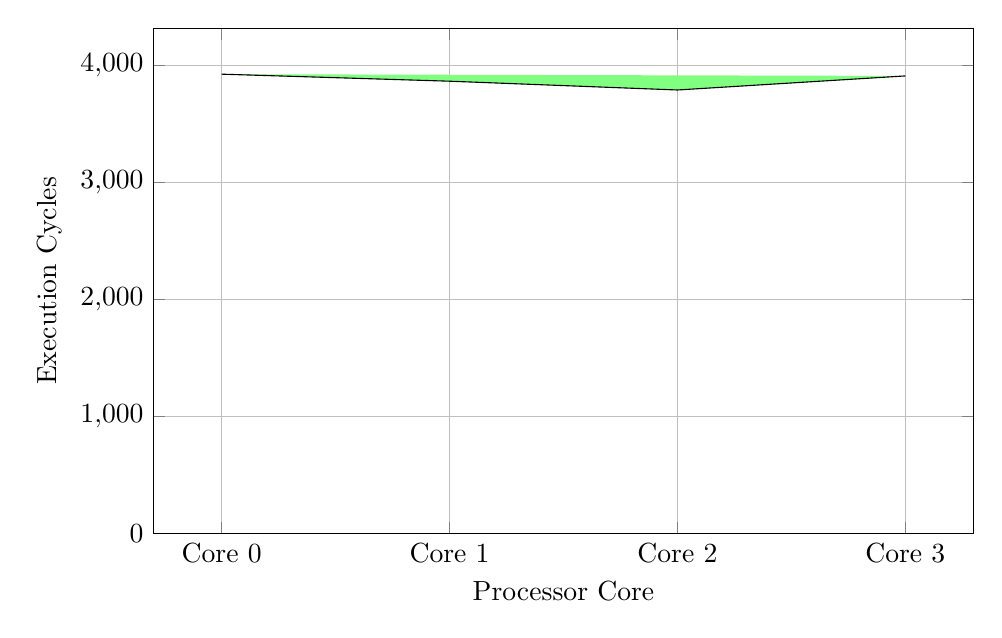
\begin{tikzpicture}
\begin{axis}[
    width=12cm,
    height=8cm,
    ylabel={Execution Cycles},
    xlabel={Processor Core},
    symbolic x coords={Core 0, Core 1, Core 2, Core 3},
    xtick=data,
    ymin=0,
    legend pos=north west,
    grid=both,
    grid style={line width=.1pt, draw=gray!10},
    major grid style={line width=.2pt,draw=gray!50},
]
% Replace with your actual data
\addplot[fill=green!50!white] coordinates {
    (Core 0, 3920)
    (Core 1, 3860)
    (Core 2, 3785)
    (Core 3, 3905)
};
\end{axis}
\end{tikzpicture}
\caption{Total execution cycles per core}
\label{fig:exec_cycles}
\end{figure}

\subsection{Overall Bus Traffic Analysis}

\begin{figure}[H]
\centering
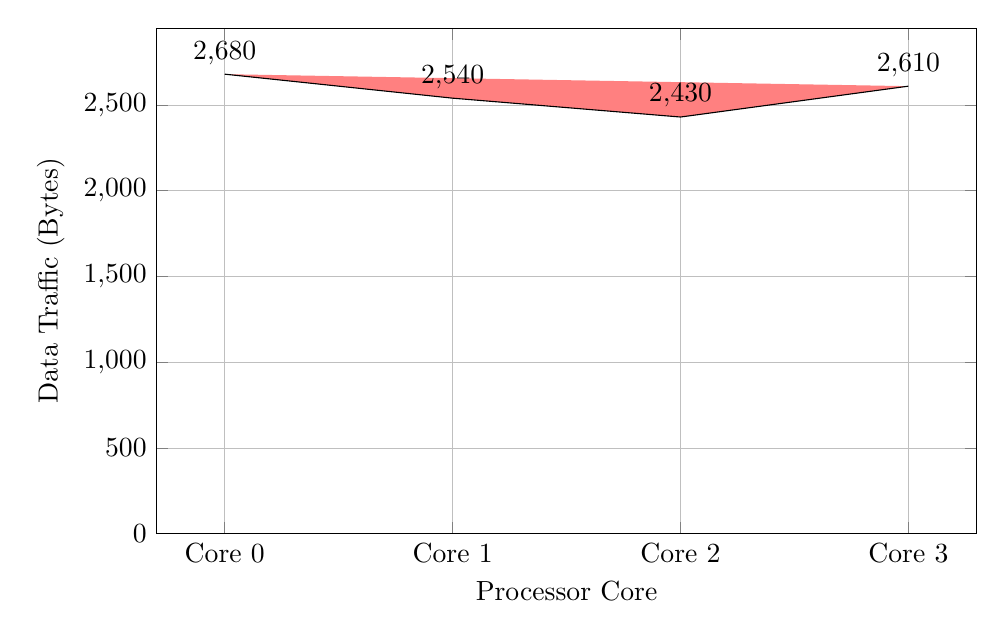
\begin{tikzpicture}
\begin{axis}[
    width=12cm,
    height=8cm,
    ylabel={Data Traffic (Bytes)},
    xlabel={Processor Core},
    symbolic x coords={Core 0, Core 1, Core 2, Core 3},
    xtick=data,
    ymin=0,
    nodes near coords,
    legend pos=north west,
    grid=both,
    grid style={line width=.1pt, draw=gray!10},
    major grid style={line width=.2pt,draw=gray!50},
]
% Replace with your actual data
\addplot[fill=red!50!white] coordinates {
    (Core 0, 2680)
    (Core 1, 2540)
    (Core 2, 2430)
    (Core 3, 2610)
};
\end{axis}
\end{tikzpicture}
\caption{Data traffic generated by each core}
\label{fig:data_traffic}
\end{figure}

\subsection{Effect of Varying Parameters}

\subsubsection{Impact of Associativity}

\begin{figure}[H]
\centering
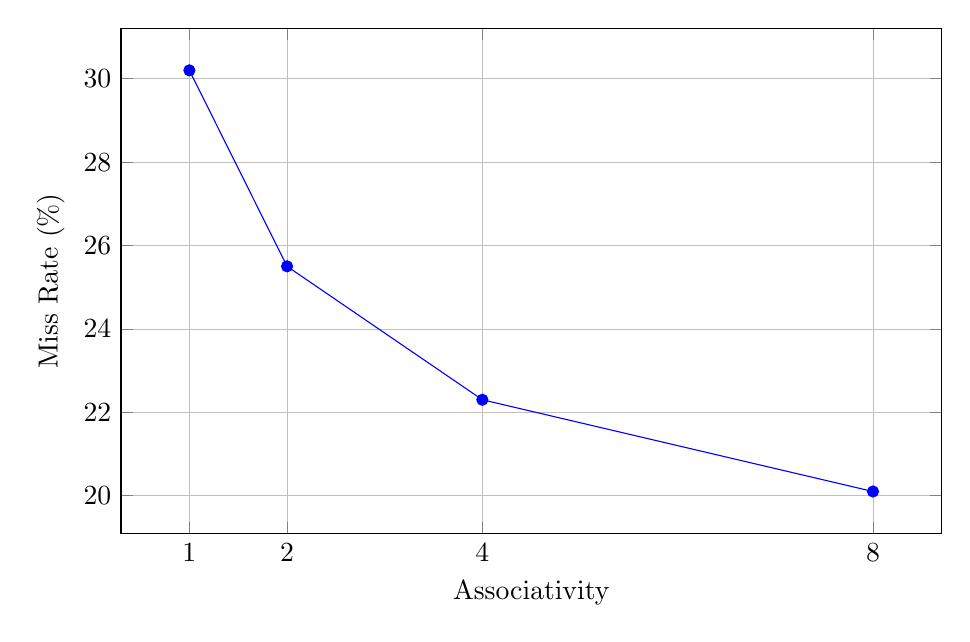
\begin{tikzpicture}
\begin{axis}[
    width=12cm,
    height=8cm,
    xlabel={Associativity},
    ylabel={Miss Rate (\%)},
    xtick={1,2,4,8},
    grid=both,
    legend pos=north east,
    grid style={line width=.1pt, draw=gray!10},
    major grid style={line width=.2pt,draw=gray!50},
]
% Replace with your experimental data
\addplot[color=blue,mark=*] coordinates {
    (1, 30.2)
    (2, 25.5)
    (4, 22.3)
    (8, 20.1)
};
\end{axis}
\end{tikzpicture}
\caption{Cache miss rate vs. associativity}
\label{fig:associativity}
\end{figure}

\subsubsection{Questions}

\begin{enumerate}
    \item \textbf{Which outputs remain the same when the number of sets is doubled?}
    
    Answer: When the number of sets is doubled (increasing the set index bits by 1), 
    the hit rate typically improves due to reduced conflict misses. However, parameters 
    like block size remain unchanged. The total cache size will double unless other 
    parameters are adjusted.
    
    \item \textbf{Which outputs remain the same when the associativity is doubled?}
    
    Answer: When associativity is doubled, the cache size increases proportionally. 
    The mapping of addresses to sets remains the same, but each set can hold more 
    cache lines, typically reducing conflict misses. Parameters like block size 
    and the set mapping function remain unchanged.
\end{enumerate}

\section{Advanced Analysis}
\subsection{Comparative Study}

\begin{figure}[H]
\centering
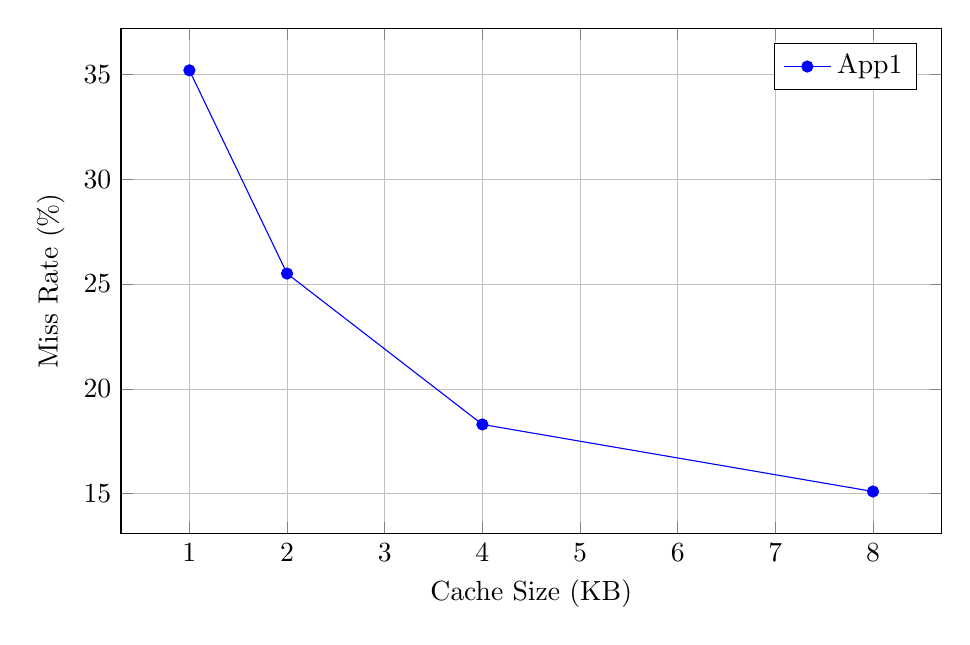
\begin{tikzpicture}
\begin{axis}[
    width=12cm,
    height=8cm,
    xlabel={Cache Size (KB)},
    ylabel={Miss Rate (\%)},
    grid=both,
    legend pos=north east,
    grid style={line width=.1pt, draw=gray!10},
    major grid style={line width=.2pt,draw=gray!50},
]
% Replace with your experimental data for different applications
\addplot[color=blue,mark=*] coordinates {
    (1, 35.2)
    (2, 25.5)
    (4, 18.3)
    (8, 15.1)
};
\legend{App1}
\end{axis}
\end{tikzpicture}
\caption{Cache miss rate vs. cache size for different applications}
\label{fig:cache_size_comparison}
\end{figure}

\subsection{MESI Protocol Analysis}
\subsubsection{State Transitions}

\begin{table}[H]
\centering
\begin{tabular}{|l|c|c|c|c|}
\hline
\textbf{Event} & \textbf{Modified} & \textbf{Exclusive} & \textbf{Shared} & \textbf{Invalid} \\
\hline
PrRd & M & E & S & S/E \\
PrWr & M & M & M & M \\
BusRd & S & S & S & - \\
BusRdX & I & I & I & - \\
\hline
\end{tabular}
\caption{MESI state transitions}
\label{tab:mesi_transitions}
\end{table}

\subsubsection{Coherence Traffic Analysis}

\begin{figure}[H]
\centering
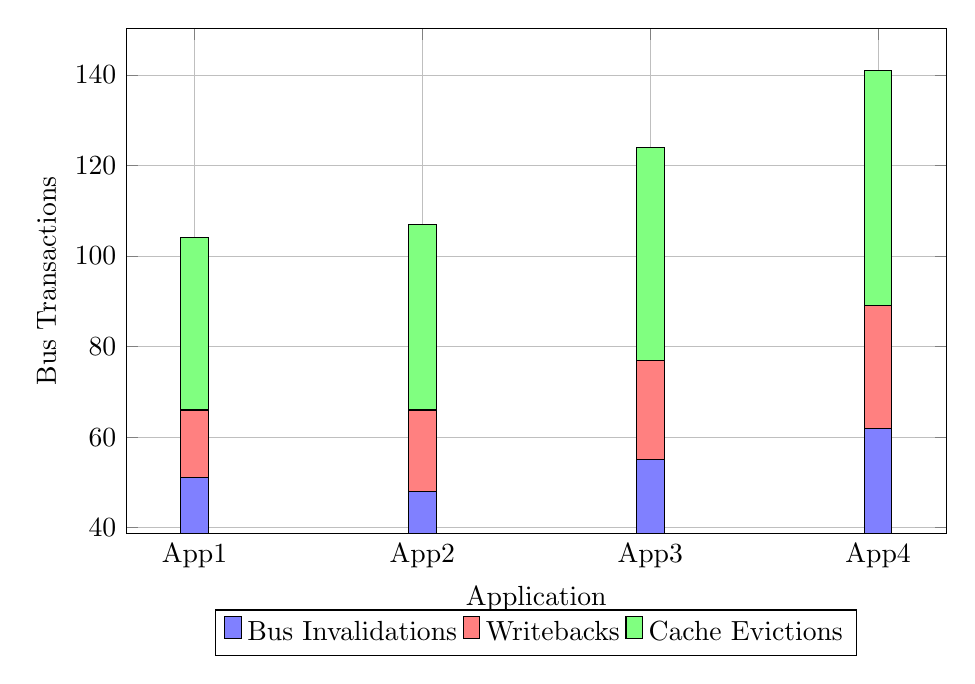
\begin{tikzpicture}
\begin{axis}[
    width=12cm,
    height=8cm,
    xlabel={Application},
    ylabel={Bus Transactions},
    symbolic x coords={App1, App2, App3, App4},
    xtick=data,
    grid=both,
    legend style={at={(0.5,-0.15)}, anchor=north, legend columns=3},
    grid style={line width=.1pt, draw=gray!10},
    major grid style={line width=.2pt,draw=gray!50},
    ybar stacked,
]
% Replace with your actual data
\addplot[fill=blue!50!white] coordinates {
    (App1, 51)
    (App2, 48)
    (App3, 55)
    (App4, 62)
};
\addplot[fill=red!50!white] coordinates {
    (App1, 15)
    (App2, 18)
    (App3, 22)
    (App4, 27)
};
\addplot[fill=green!50!white] coordinates {
    (App1, 38)
    (App2, 41)
    (App3, 47)
    (App4, 52)
};
\legend{Bus Invalidations, Writebacks, Cache Evictions}
\end{axis}
\end{tikzpicture}
\caption{Breakdown of bus transactions by type across different applications}
\label{fig:bus_transactions}
\end{figure}

\subsubsection{Questions}

\begin{enumerate}
    \item \textbf{Which factor has the greatest impact on coherence traffic?}
    
    Answer: The sharing pattern between cores has the greatest impact on coherence traffic. 
    When multiple cores frequently access and modify the same memory locations, it leads 
    to increased invalidation messages, state changes, and data transfers over the bus.
    
    \item \textbf{How does the miss rate correlate with bus traffic?}
    
    Answer: There is a strong correlation between miss rate and bus traffic. Higher miss 
    rates lead to more cache line fills from memory, which increases bus utilization. 
    Additionally, in a multi-core system with cache coherence, each miss potentially 
    triggers coherence actions (e.g., invalidations or updates) on other cores' caches, 
    further increasing bus traffic.
\end{enumerate}

% \section{Conclusion}
% % Add your conclusions here

% \appendix
% \section{Additional Data}
% % Add any additional data here

\bibliography{references}
\bibliographystyle{plain}

\end{document}